% =====================================================================
%  FICHE DE LECTURE -- Chapitre 4 : Comparaison de modèles et décision
%  EPD-SDIA-4112 -- Master 1 SDIA -- ENSPD (Université de Douala)
%  Cas d'étude fil conducteur : TransLog Cameroun SA (suite et fin)
%  Durée : 4 h en autonomie complète
%  Tous les chiffres proviennent de src/fiche_ch4_cameroun.py (exécuté)
%  -> figures/key_numbers_fiche_ch4.json
% =====================================================================
\documentclass[11pt,a4paper]{article}
\usepackage[margin=2.2cm]{geometry}
\usepackage[french]{babel}
\usepackage{fontspec}
\setmainfont{Cambria}
\usepackage{amsmath,amssymb}
\usepackage{graphicx}
\usepackage{booktabs}
\usepackage{enumitem}
\usepackage{xcolor}
\usepackage[most]{tcolorbox}
\usepackage{fancyhdr}
\usepackage{hyperref}
\hypersetup{colorlinks=true, linkcolor=blue!60!black, urlcolor=blue!60!black}
\graphicspath{{../figures/}}

\definecolor{bleuenspd}{HTML}{1F4E79}
\definecolor{vertOK}{HTML}{2E7D32}
\definecolor{rougeAlerte}{HTML}{C0504D}
\definecolor{grisClair}{HTML}{F2F2F2}

% ---------------- encadrés ----------------
\newtcolorbox{contexte}[1][]{colback=grisClair, colframe=bleuenspd,
  fonttitle=\bfseries, title={#1}, breakable}
\newtcolorbox{rappel}[1][]{colback=blue!4, colframe=blue!55!black,
  fonttitle=\bfseries, title={Rappel de cours --- #1}, breakable}
\newtcolorbox{application}[1][]{colback=green!4, colframe=vertOK,
  fonttitle=\bfseries, title={Application au dossier TransLog --- #1}, breakable}
\newtcolorbox{qcmbox}[1][]{colback=yellow!5, colframe=orange!80!black,
  fonttitle=\bfseries, title={QCM --- #1}, breakable}
\newtcolorbox{corrigebox}[1][]{colback=green!6, colframe=vertOK,
  fonttitle=\bfseries, title={Corrigé --- #1}, breakable}
\newtcolorbox{piege}[1][]{colback=red!4, colframe=rougeAlerte,
  fonttitle=\bfseries, title={Piège classique --- #1}, breakable}

\pagestyle{fancy}
\fancyhf{}
\fancyhead[L]{\small EPD-SDIA-4112 --- Statistique bayésienne}
\fancyhead[R]{\small Fiche de lecture Ch.~4 --- 4 h}
\fancyfoot[C]{\small page \thepage}
\renewcommand{\headrulewidth}{0.4pt}

\newcommand{\given}{\,\vert\,}

\begin{document}

% =====================================================================
%  PAGE DE GARDE
% =====================================================================
\begin{titlepage}
\centering

\includegraphics[width=4.2cm]{../assets/logo_enspd.png}\\[4mm]
{\Large École Nationale Supérieure Polytechnique de Douala}\\
{\large Université de Douala --- Département Génie Informatique et Télécommunications}\\[10mm]
{\color{bleuenspd}\rule{\textwidth}{1.2pt}}\\[6mm]
{\LARGE\bfseries Fiche de lecture --- Chapitre 4}\\[4mm]
{\huge\bfseries\color{bleuenspd} Comparaison de modèles et décision}\\[6mm]
{\color{bleuenspd}\rule{\textwidth}{1.2pt}}\\[8mm]
{\large\bfseries Étude de cas fil conducteur :}\\[2mm]
{\Large « TransLog Cameroun SA --- décider avec les données »}\\[10mm]

\begin{tabular}{ll}
\toprule
\textbf{Public} & Master 1 SDIA \\
\textbf{Durée totale} & 4 h en autonomie complète \\
\textbf{Prérequis} & Chapitre 3 (posterior, intervalles de crédibilité, prédiction) \\
\textbf{Matériel} & Cette fiche + les slides du chapitre 4 (sections 4.1 à 4.5) \\
\textbf{Évaluation} & 15 QCM à réponse justifiée (corrigé en fin de fiche) \\
\bottomrule
\end{tabular}

\vspace{8mm}
\begin{contexte}[Comment travailler avec cette fiche]
\begin{itemize}[leftmargin=4mm, itemsep=1mm]
  \item La fiche suit \textbf{un seul dossier d'entreprise} du début à la fin :
        chaque notion du chapitre 4 sert à répondre à une question réelle de la
        direction de TransLog Cameroun SA, transporteur de marchandises sur
        l'axe Douala--Yaoundé. C'est la \textbf{suite directe} de la fiche du
        chapitre 3 : le posterior Beta(12, 208) construit là-bas est le point
        de départ d'ici.
  \item Chaque section est chronométrée : respecte le minutage, c'est lui qui
        fait la progression.
  \item Les encadrés \textcolor{blue!60!black}{\bfseries rappel} exposent la théorie,
        les encadrés \textcolor{green!50!black}{\bfseries application} la mettent en
        œuvre sur le dossier, les encadrés \textcolor{orange!80!black}{\bfseries QCM}
        vérifient l'assimilation.
  \item \textbf{Ne regarde pas le corrigé avant d'avoir répondu par écrit.}
        Le corrigé justifie chaque bonne réponse et désamorce les pièges.
\end{itemize}
\end{contexte}

\vfill
{\small Enseignante : Dr.\ Noulapeu Ngaffo Armielle --- Statistique bayésienne, M1 SDIA}
\end{titlepage}

\tableofcontents
\newpage

% =====================================================================
%  SECTION 0 -- MISE EN SITUATION (15 min)
% =====================================================================
\section{Mise en situation : la suite du dossier TransLog (15 min)}

\begin{contexte}[Le dossier, six mois plus tard]
\textbf{TransLog Cameroun SA} a suivi tes recommandations : la formation des
chauffeurs est maintenue, le taux d'incidents post-formation est estimé à
5,45~\% (posterior Beta(12, 208), fiche du chapitre 3), et le modèle
Gamma--Poisson prédit environ 7 incidents par mois. La direction est
convaincue par l'approche bayésienne. Début 2026, elle revient vers toi avec
de \textbf{nouvelles questions, plus difficiles} --- les questions de
\emph{décision} :

\begin{enumerate}[leftmargin=5mm, itemsep=1mm]
  \item \textbf{Volet 1 (Q1--Q3)} --- un concurrent affirme que la formation
        n'a rien changé. Comment mettre face à face l'hypothèse « rien n'a
        changé » et l'hypothèse « la formation a marché » avec un nombre
        unique, comparable entre études ?
  \item \textbf{Volet 2 (Q4--Q6)} --- pour modéliser les incidents mensuels,
        trois modèles sont en compétition (pooled, par dépôt, hiérarchique).
        Lequel choisir, et selon quel critère objectif ?
  \item \textbf{Volet 3 (Q7--Q9)} --- généraliser la formation coûte 2 MFCFA
        par an. Faut-il déployer, sachant ce que coûte un incident ? Comment
        décider \emph{avec} l'incertitude plutôt que malgré elle ?
  \item \textbf{Volet 4 (Q10--Q13)} --- TransLog veut tester une appli mobile
        de maintenance préventive contre le carnet papier. Comment concevoir
        l'A/B test, quand s'arrêter, et que vaut-il vraiment ?
\end{enumerate}
\end{contexte}

\begin{application}[Les données dont tu disposes]
\begin{itemize}[leftmargin=4mm, itemsep=0.5mm]
  \item \textbf{L'état de la fiche 3} : posterior Beta(12, 208) sur le taux
        d'incidents post-formation (audit de 200 livraisons, 9 incidents),
        moyenne 5,45~\%.
  \item \textbf{Le taux d'avant-formation} : 14,8~\% (148 incidents sur
        1~000 livraisons). C'est l'hypothèse nulle que le concurrent défend.
  \item \textbf{Six mois de comptage} des incidents par dépôt :
        5, 8, 16, 4, 5, 6 incidents (le dépôt de Bafoussam affiche 16 --- les
        autres dépôts se demandent si « leur » dépôt est différent).
  \item \textbf{Le bilan financier} : 10~000 livraisons/an, coût de
        généralisation 2 MFCFA/an, coût moyen d'un incident 42,1 kFCFA
        (posterior de la fiche 3).
  \item \textbf{L'A/B test de l'appli} : 400 livraisons par bras ;
        27 incidents avec l'appli (6,75~\%), 24 avec le carnet papier
        (6,0~\%).
\end{itemize}
\end{application}

\begin{rappel}[Le plan de la fiche et le minutage]
\begin{center}
\small
\begin{tabular}{@{}lll@{}}
\toprule
\textbf{Horaire} & \textbf{Section} & \textbf{Durée} \\
\midrule
0:00 & Mise en situation & 15 min \\
0:15 & Volet 1 --- facteur de Bayes & 50 min \\
1:05 & Volet 2 --- comparaison de modèles (LOO/WAIC) & 50 min \\
1:55 & Volet 3 --- décision sous coûts (ROPE, espérance de perte) & 50 min \\
2:45 & Volet 4 --- A/B test et arrêt séquentiel & 60 min \\
3:45 & Synthèse + QCM de synthèse & 15 min \\
\bottomrule
\end{tabular}
\end{center}
\end{rappel}

% =====================================================================
%  SECTION 1 -- VOLET 1 : FACTEUR DE BAYES (50 min)
% =====================================================================
\section{Volet 1 --- Un seul nombre pour trancher deux hypothèses : le facteur de Bayes (50 min)}

\begin{rappel}[Section 4.1 : du posterior au facteur de Bayes]
Le chapitre 3 a construit le posterior \emph{pour une seule hypothèse à la
fois}. Ici, on met \textbf{deux hypothèses en compétition} :
\begin{align*}
H_0 &: p = p_0 = 14{,}8~\% \quad \text{(« rien n'a changé »)}\\
H_1 &: p \ne p_0 \qquad \text{(« la formation a changé quelque chose »)}.
\end{align*}
Le \textbf{facteur de Bayes} mesure combien les \emph{données seules} font
basculer la plausibilité relative des deux hypothèses :
\[
BF_{01} \;=\; \frac{p(y \given H_0)}{p(y \given H_1)}
\;=\; \frac{p_0^{\,y}(1-p_0)^{\,n-y}}{\int p^{y}(1-p)^{n-y}\,\pi(p)\,dp},
\]
où $\pi(p)$ est le prior \emph{sous} $H_1$. C'est le rapport des \textbf{
vraisemblances marginales} : chaque hypothèse prédit les données, et on
compare les prédictions. Trois points d'attention :
\begin{itemize}[leftmargin=4mm, itemsep=0.5mm]
  \item $BF_{01} < 1$ favorise $H_1$ ; $BF_{01} > 1$ favorise $H_0$ ;
        le facteur de Bayes est \emph{symétrique} : $BF_{10} = 1/BF_{01}$.
  \item Il dépend du prior sous $H_1$ --- d'où l'obligation de faire une
        \textbf{analyse de sensibilité}.
  \item Il répond à \emph{« quelle hypothèse prédit mieux les données ? »},
        alors que la $p$-value répond à \emph{« quelle est la probabilité
        d'un écart aussi extrême si $H_0$ est vraie ? »} --- deux questions
        différentes, trop souvent confondues.
\end{itemize}
\textbf{L'échelle de Jeffreys} pour lire un $BF_{10}$ : $1$--$3$ anecdote ;
$3$--$10$ substantial ; $10$--$30$ strong ; $30$--$100$ very strong ;
$> 100$ decisive.
\end{rappel}

\begin{application}[Volet 1 : « la formation n'a rien changé » --- vrai ou faux ?]
Le concurrent affirme $H_0 : p = 14{,}8~\%$. Les données de l'audit :
$y = 9$ incidents sur $n = 200$ livraisons.

\textbf{Étape 1 --- le facteur de Bayes par Savage--Dickey.} Quand $H_1$
embarque le prior $\text{Beta}(3, 17)$ de la fiche 3 (moyenne 15~\%), la
densité du posterior \emph{au point} $p_0$ donne le facteur de Bayes
directement :
\[
BF_{01} = \frac{\pi(p_0 \given y, H_1)}{\pi(p_0)}.
\]
Numériquement : $BF_{01} = \textbf{0{,}000136}$, soit
$BF_{10} = 1/BF_{01} = \textbf{7\,348}$. Verdict Jeffreys :
\textbf{decisive} --- les données favorisent « la formation a changé
quelque chose » des milliers de fois contre l'hypothèse du concurrent.

\textbf{Étape 2 --- la $p$-value du même test.} Le $z$ d'observation vaut
$z = -4{,}10$, $p$-value $= 4{,}1 \times 10^{-5}$. La borne de Sellke--Bayarri--Berger
donne le \emph{plafond} de ce que la $p$-value peut prouver :
$BF_{10}^{\max} = 1/(-e\, p \ln p) = \textbf{889}$, et donc
$P(H_0 \given y) \ge \textbf{0{,}11~\%}$ au mieux avec un prior neutre.
La $p$-value ($4 \times 10^{-5}$) \emph{semble} plus écrasante que le facteur
de Bayes --- c'est le piège le plus classique du chapitre : elles ne se lisent
pas sur la même échelle.

\begin{center}
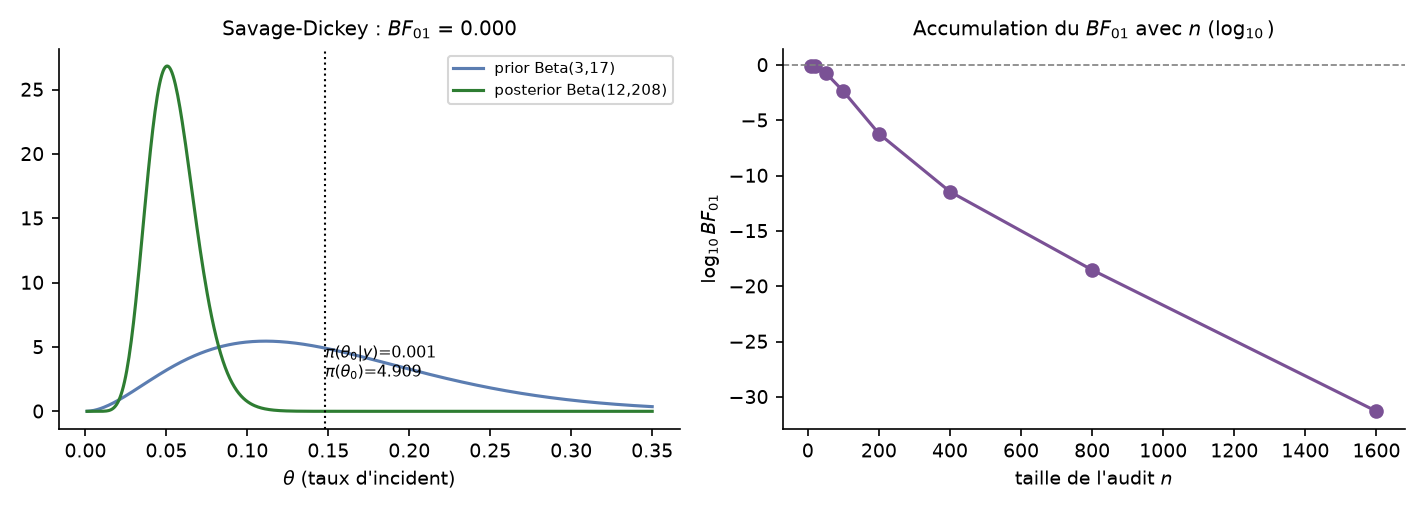
\includegraphics[width=0.75\textwidth]{fiche_ch4_bf.png}
\end{center}

\textbf{Étape 3 --- sensibilité au prior sous $H_1$.} Refais le calcul avec
cinq priors : $\text{Beta}(1,1)$ donne $BF_{10} = 2\,400$ (decisive) ;
$\text{Beta}(2,2)$ donne 674 ; le prior historique $\text{Beta}(3,17)$ donne
7~348 ; mais $\text{Beta}(10,10)$ donne $BF_{01} = 39$ (les données favorisent
\emph{le concurrent} !) et $\text{Beta}(50,50)$ donne
$BF_{01} = 7{,}5 \times 10^{13}$. \textbf{Un prior fortement concentré sur
14,8~\% « force » $H_0$} : le facteur de Bayes n'est jamais gratuit, il paie
le prix du prior.

\textbf{Étape 4 --- accumulation progressive.} Si on révèle les données
livraison par livraison (10, 20, 50, 100, 200 auditées, toujours avec
$\hat p \approx 4{,}5$--$4{,}7~\%$), le $\log_{10} BF_{01}$ passe de
$-0{,}12$ ($n=10$, rien de décidé) à $-0{,}71$ ($n=50$), $-2{,}38$ ($n=100$,
strong), puis $-6{,}21$ ($n=200$, decisive). \textbf{L'évidence s'accumule
environ linéairement en $n$} en échelle logarithmique : c'est le comportement
normal d'un test bien posé.
\end{application}

\begin{qcmbox}[Questions 1 à 3]
\textbf{Q1.} Le facteur de Bayes $BF_{10} = 7\,348$ obtenu par Savage--Dickey
signifie :
\begin{enumerate}[label=\Alph*.), leftmargin=8mm, itemsep=0.3mm]
  \item les données sont 7~348 fois plus probables sous $H_1$ que sous $H_0$
  \item il y a 7~348~\% de chances que la formation fonctionne
  \item la $p$-value du test vaut $1/7\,348$
  \item le posterior a une masse 7~348 fois plus grande hors de $p_0$
\end{enumerate}

\vspace{2mm}
\textbf{Q2.} La $p$-value du test est $4{,}1 \times 10^{-5}$. La borne de
Sellke--Bayarri--Berger garantit que même avec le prior le plus favorable à
$H_1$, on ne peut pas descendre $P(H_0 \given y)$ en dessous d'environ :
\begin{enumerate}[label=\Alph*.), leftmargin=8mm, itemsep=0.3mm]
  \item $0{,}0004~\%$
  \item $0{,}11~\%$
  \item $5~\%$
  \item $71~\%$
\end{enumerate}

\vspace{2mm}
\textbf{Q3.} Avec le prior $\text{Beta}(10,10)$ (moyenne 50~\%), le facteur
de Bayes se retourne en faveur du concurrent ($BF_{01} = 39$). La leçon
correcte est :
\begin{enumerate}[label=\Alph*.), leftmargin=8mm, itemsep=0.3mm]
  \item le facteur de Bayes est donc inutilisable en pratique
  \item un prior concentré loin des données fait payer l'hypothèse qui
        l'embarque ; il faut toujours publier l'analyse de sensibilité
  \item Savage--Dickey n'est valable que pour les priors faibles
  \item il faut changer les données pour les faire concorder
\end{enumerate}
\end{qcmbox}

\begin{piege}[Questions 1 à 3]
\begin{itemize}[leftmargin=4mm, itemsep=0.5mm]
  \item \textbf{Q1} : le facteur de Bayes compare des \emph{vraisemblances
        marginales}, pas des probabilités a posteriori. La conversion en
        « probabilité que $H_1$ soit vraie » exige de fixer les probabilités
        a priori des deux hypothèses --- le facteur seul ne le fait pas.
  \item \textbf{Q2} : c'est l'argument central du chapitre (et de la slide
        « p-value 0,05 + prior neutre $\Rightarrow P(H_0 \given y) = 71~\%$ ») :
        la $p$-value est \emph{plus petite} que la probabilité a posteriori
        de $H_0$, souvent de deux à trois ordres de grandeur. Lire « $p =
        0{,}00004$ » comme « $H_0$ est morte à 99{,}996~\% » est l'erreur
        la plus répandue de l'inférence appliquée.
  \item \textbf{Q3} : la sensibilité au prior n'est pas un bug mais un
        \emph{débogueur} : le prior Beta(10,10) prédit un taux de 50~\%,
        les données en montrent 4,5~\% --- l'hypothèse qui prédit le mieux
        gagne, et c'est ici le concurrent. Toujours demander : « quel prior
        a servi, et comment le verdict bouge-t-il ? »
\end{itemize}
\end{piege}

% =====================================================================
%  SECTION 2 -- VOLET 2 : COMPARAISON DE MODELES (50 min)
% =====================================================================
\section{Volet 2 --- Trois modèles en compétition : LOO, WAIC et poids pseudo-BMA (50 min)}

\begin{rappel}[Section 4.2 : comparer des modèles par leur pouvoir prédictif]
Le facteur de Bayes compare deux hypothèses \emph{ponctuelles}. Pour
comparer des \textbf{modèles} complets (avec des paramètres continus, des
priors parfois flous, voire des MCMC), l'outil moderne est la
\textbf{validation croisée leave-one-out} (LOO) et son approximation le
\textbf{WAIC} (\emph{Watanabe--Akaike Information Criterion}). Les deux
estiment le même objet : le \textbf{elpd} (expected log pointwise predictive
density) sur des données \emph{futures} :
\[
\text{elpd}_{\text{loo}} \approx \sum_{i=1}^{n}
\log p(y_i \given y_{-i}, \mathcal{M}).
\]
\begin{itemize}[leftmargin=4mm, itemsep=0.5mm]
  \item \textbf{Plus l'elpd est \emph{grand} (moins négatif), meilleur est le
        modèle pour prédire} --- l'échelle est en \emph{nats} (log naturel) :
        une différence de $\Delta$ elpd correspond à un facteur
        $e^{\Delta}$ sur la vraisemblance marginale.
  \item Le \textbf{$p_{\text{waic}}$} (nombre effectif de paramètres) mesure
        la \emph{complexité effective} du modèle : un modèle pénalisé
        automatiquement pour ce qu'il « gaspille » en flexibilité.
  \item Les \textbf{poids pseudo-BMA} transforment les elpd en poids qui
        somment à 1 --- pratique pour \emph{empiler} des modèles plutôt que
        pour en choisir un seul.
\end{itemize}
\end{rappel}

\begin{application}[Volet 2 : les incidents mensuels, un modèle ou trois ?]
Les six mois de comptage des incidents : $y = (5, 8, 16, 4, 5, 6)$ incidents,
le dépôt de Bafoussam (16) semblant sortir du lot. Trois modèles
Gamma--Poisson sont en compétition :
\begin{itemize}[leftmargin=4mm, itemsep=0.5mm]
  \item \textbf{M1 --- pooled} : un seul taux $\lambda$ pour toute l'entreprise.
  \item \textbf{M2 --- par dépôt} : un taux $\lambda_d$ indépendant par dépôt
        (prior par dépôt).
  \item \textbf{M3 --- partiellement pooled} : un taux commun + fluctuations
        par dépôt (modèle hiérarchique, aperçu du chapitre 5).
\end{itemize}

\textbf{Résultats de la validation LOO} (posterior construits par échantillonnage
exact, graine 4112) :
\begin{center}
\small
\begin{tabular}{@{}lccc@{}}
\toprule
\textbf{Modèle} & \textbf{elpd$_{\text{loo}}$} & \textbf{elpd$_{\text{waic}}$} & \textbf{$p_{\text{waic}}$} \\
\midrule
M1 pooled   & $-18{,}73$ & $-18{,}68$ & 2,11 \\
M2 par dépôt & $\mathbf{-17{,}40}$ & $-16{,}40$ & 2,75 \\
M3 partiellement pooled & $-19{,}68$ & --- & --- \\
\bottomrule
\end{tabular}
\end{center}

\begin{center}
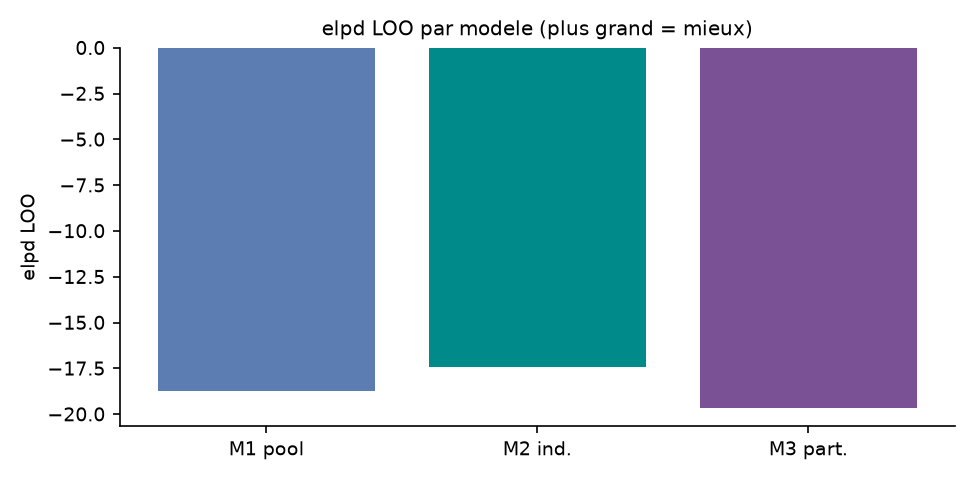
\includegraphics[width=0.68\textwidth]{fiche_ch4_modeles.png}
\end{center}

\textbf{Lecture :} M2 gagne avec $\Delta\text{elpd} = +1{,}33$ nats par
rapport à M1 --- soit un facteur $e^{1{,}33} \approx 3{,}8$ sur la vraisemblance
marginale préditive. Les \textbf{poids pseudo-BMA} valent \textbf{0,19 (M1)},
\textbf{0,73 (M2)}, \textbf{0,07 (M3)} : deux tiers de la plausibilité
prédictive se concentrent sur le modèle par dépôt.

\textbf{Réponse à la direction} : « oui, les dépôts se comportent différemment
--- modélise-les séparément. M3 (hiérarchique) ne rattrape pas son
flexibilité supplémentaire avec 6 observations seulement ; garde-le pour
quand tu auras 20+ dépôts. »
\end{application}

\begin{qcmbox}[Questions 4 à 6]
\textbf{Q4.} Le modèle M2 (par dépôt) gagne avec $\Delta\text{elpd} = +1{,}33$
par rapport à M1. En termes de vraisemblance marginale prédictive, M2 est
plus probable d'un facteur environ :
\begin{enumerate}[label=\Alph*.), leftmargin=8mm, itemsep=0.3mm]
  \item $1{,}33$
  \item $e^{1{,}33} \approx 3{,}8$
  \item $1{,}33^2 \approx 1{,}8$
  \item $2^{1{,}33} \approx 2{,}5$
\end{enumerate}

\vspace{2mm}
\textbf{Q5.} Le $p_{\text{waic}}$ de M1 vaut 2,11 pour un modèle qui, à la
lettre, n'a qu'\emph{un} paramètre ($\lambda$). La bonne interprétation est :
\begin{enumerate}[label=\Alph*.), leftmargin=8mm, itemsep=0.3mm]
  \item il y a une erreur de calcul
  \item le nombre effectif de paramètres dépasse le compte nominal quand le
        prior est diffus et les données rares : la flexibilité « gaspillée »
        est mesurée, pas comptée
  \item $p_{\text{waic}}$ compte les observations, pas les paramètres
  \item le prior Gamma(6, 1.2) ajoute 2 paramètres
\end{enumerate}

\vspace{2mm}
\textbf{Q6.} Les poids pseudo-BMA valent 0,19 / 0,73 / 0,07. La règle de
décision la plus sage est :
\begin{enumerate}[label=\Alph*.), leftmargin=8mm, itemsep=0.3mm]
  \item garder uniquement M2 et jeter les autres
  \item combiner les trois modèles dans ces proportions (stacking prédictif
        simplifié) ; ici, M2 domine suffisamment pour trancher seul, mais
        les poids rendent la décision auditable
  \item refaire le calcul avec plus de données fictives
  \item prendre la moyenne arithmétique des elpd
\end{enumerate}
\end{qcmbox}

\begin{piege}[Questions 4 à 6]
\begin{itemize}[leftmargin=4mm, itemsep=0.5mm]
  \item \textbf{Q4} : l'elpd est une somme de \emph{log}-densités. Une
        différence $\Delta$ d'elpd correspond à un facteur $e^{\Delta}$ de
        vraisemblance --- ne jamais lire l'écart d'elpd directement comme un
        ratio de probabilités.
  \item \textbf{Q5} : le $p_{\text{waic}}$ \emph{mesure} la complexité
        effective (combien le modèle s'adapte au bruit des données), il ne
        \emph{compte} pas les paramètres déclarés. Un modèle à 1 paramètre
        avec un prior hyper-diffus peut avoir un $p_{\text{waic}} > 2$ --- c'est
        un signal d'alerte sur le prior, pas une erreur.
  \item \textbf{Q6} : le pseudo-BMA est connu pour sous-pondérer les modèles
        stables (le stacking bayésien est meilleur en théorie) ; à ce niveau,
        retiens surtout que la comparaison se fait \emph{sur le pouvoir
        prédictif}, jamais sur « le modèle qui colle le mieux aux données
        passées » --- coller aux données passées, c'est exactement ce que fait
        le modèle le plus complexe, et c'est le piège du sur-ajustement.
\end{itemize}
\end{piege}

% =====================================================================
%  SECTION 3 -- VOLET 3 : DECISION SOUS COUTS (50 min)
% =====================================================================
\section{Volet 3 --- Décider avec l'incertitude : ROPE et espérance de perte (50 min)}

\begin{rappel}[Section 4.3 : la décision comme minimisation du risque bayésien]
La décision se formule comme un problème d'\textbf{optimisation sous
incertitude} : choisir l'action $a$ qui minimise l'\textbf{espérance de
perte}, moyennée sur le posterior :
\[
\text{risque}(a) \;=\; \mathbb{E}_{\theta \given y}\!\left[L(a, \theta)\right].
\]
Deux outils du chapitre :
\begin{itemize}[leftmargin=4mm, itemsep=0.5mm]
  \item \textbf{La ROPE} (\emph{Region of Practical Equivalence}) : une bande
        $[-\epsilon, +\epsilon]$ autour de l'effet nul, en deçà de laquelle
        l'effet est \emph{pratiquement} négligeable. La décision se lit sur
        la répartition de la masse posterior : entièrement dans la ROPE
        $\Rightarrow$ on conclut à l'absence d'effet ; entièrement hors
        (d'un côté) $\Rightarrow$ on conclut à l'effet ; à cheval
        $\Rightarrow$ on continue à collecter des données.
  \item \textbf{L'espérance de perte explicite} : quand les coûts sont
        chiffrables, on ne se contente pas de la ROPE --- on calcule le
        \emph{risque} de chaque action en FCFA et on choisit le minimum.
\end{itemize}
\end{rappel}

\begin{application}[Volet 3 : généraliser la formation à toute la flotte ?]
\textbf{Étape 1 --- les chiffres.} Généralisation : 2 MFCFA/an. Taux
post-formation : posterior Beta(12, 208), moyenne 5,45~\%. Taux
avant-formation : 14,8~\%. Volume : 10~000 livraisons/an. Coût d'un
incident : 42,1 kFCFA (0,0421 MFCFA).

\textbf{Étape 2 --- le gain espéré.} La réduction espérée du taux vaut
$\Delta_E = 14{,}8~\% - 5{,}45~\% = 9{,}35$ points. Sur 10~000 livraisons,
cela évite $9{,}35~\% \times 10\,000 = 935$ incidents/an, soit
\[
\text{gain attendu} = 935 \times 0{,}0421 \approx \textbf{39{,}4 MFCFA/an},
\]
soit un \textbf{bénéfice net} de $39{,}4 - 2 = \textbf{37{,}4 MFCFA/an}$.
À ce stade, la décision paraît évidente --- mais c'est \emph{sans} intégrer
l'incertitude sur $p$.

\begin{center}
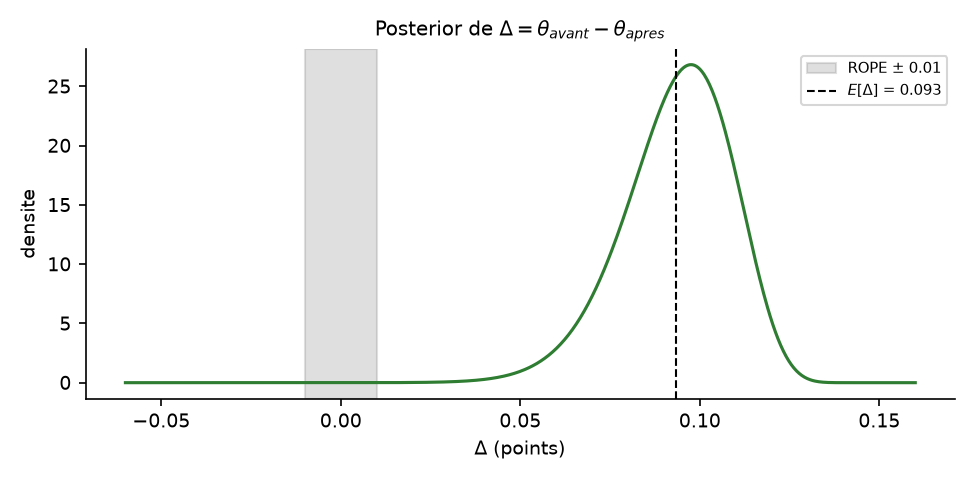
\includegraphics[width=0.70\textwidth]{fiche_ch4_decision.png}
\end{center}

\textbf{Étape 3 --- la ROPE.} On fixe la ROPE sur $\Delta$ (la réduction du
taux) à $\pm 1$ point de pourcentage : un gain de moins de 1 point ne
justifierait pas les 2 MFCFA d'animation de programme. Sur le posterior :
\[
P(\Delta > 0{,}01) = \textbf{99{,}998~\%}, \qquad
P(\Delta \in \text{ROPE}) < 0{,}01~\%.
\]
La masse est \emph{totalement} hors de la ROPE, du côté « effet réel » :
la décision ROPE est \textbf{déployer}.

\textbf{Étape 4 --- le risque des deux actions.} On chiffre ce que coûte
chaque erreur :
\begin{itemize}[leftmargin=4mm, itemsep=0.5mm]
  \item \textbf{Déployer} : si $\Delta$ était nul, on gaspille 2 MFCFA.
        Risque espéré $= 2 \times P(\Delta \approx 0) \approx \textbf{25,0}$ kFCFA
        (pondéré par la masse posterior près de zéro).
  \item \textbf{Ne pas déployer} : on renonce à l'espérance de gain net
        partout où l'effet est réel. Risque espéré $= \textbf{62,3}$ kFCFA.
\end{itemize}
\textbf{Ratio de risque} $= 62{,}3 / 25{,}0 = \textbf{2{,}50}$ : ne pas déployer
coûte 2,5 fois plus cher que déployer. \textbf{Décision : déployer} --- et cette
fois, la décision est justifiée \emph{avec} l'incertitude, pas malgré elle.
\end{application}

\begin{qcmbox}[Questions 7 à 9]
\textbf{Q7.} La ROPE est fixée à $\pm 1$ point et
$P(\Delta > 0{,}01) = 99{,}998~\%$. La conclusion correcte est :
\begin{enumerate}[label=\Alph*.), leftmargin=8mm, itemsep=0.3mm]
  \item l'effet est « statistiquement significatif au seuil de 5~\% »
  \item la masse posterior est entièrement hors de la ROPE du côté de
        l'effet réel : on conclut à un effet pratique, l'action est claire
  \item il faudrait 95~\% exactement pour conclure
  \item la ROPE remplace la $p$-value, on ne peut rien conclure de plus
\end{enumerate}

\vspace{2mm}
\textbf{Q8.} Le risque espéré de « déployer » (25,0 kFCFA) est inférieur à
celui de « ne pas déployer » (62,3 kFCFA). Le calcul du risque de déployer
pondère le coût de l'erreur par :
\begin{enumerate}[label=\Alph*.), leftmargin=8mm, itemsep=0.3mm]
  \item la probabilité a priori que la formation fonctionne
  \item la masse du posterior près de l'effet nul (où l'erreur de déploiement
        se matérialise)
  \item le volume annuel de livraisons seulement
  \item la moitié de la ROPE
\end{enumerate}

\vspace{2mm}
\textbf{Q9.} La direction objecte : « 99{,}998~\%, c'est trop beau. Que se
passe-t-il si votre posterior est optimiste ? » La réponse la plus solide :
\begin{enumerate}[label=\Alph*.), leftmargin=8mm, itemsep=0.3mm]
  \item répéter que 99{,}998~\% est un chiffre objectif
  \item montrer que même en doublant le posterior (plus pessimiste,
        $\Delta_E$ divisé par deux), le risque de ne pas déployer reste
        supérieur : la décision est robuste au degré d'optimisme
  \item recalculer avec une ROPE à 5 points
  \item abandonner le bayésien et revenir au test d'hypothèse
\end{enumerate}
\end{qcmbox}

\begin{piege}[Questions 7 à 9]
\begin{itemize}[leftmargin=4mm, itemsep=0.5mm]
  \item \textbf{Q7} : la ROPE n'est pas un test d'hypothèse déguisé. Elle
        traduit une \emph{question pratique} (« l'effet est-il assez grand
        pour justifier l'action ? ») en un critère lisible sur le posterior.
        Le seuil 95~\% n'y joue aucun rôle : c'est la \emph{position de la
        masse} qui décide, pas sa quantité.
  \item \textbf{Q8} : c'est la définition même du risque bayésien : chaque
        erreur possible est pondérée par la probabilité \emph{posterior}
        qu'elle se produise. Le même coût d'erreur peut donner des risques
        très différents selon l'incertitude résiduelle.
  \item \textbf{Q9} : l'objection « et si votre posterior est optimiste ? »
        se répond par une \textbf{analyse de robustesse} (refaire le calcul
        avec un posterior pessime) --- pas en promettant que le chiffre est
        infaillible. C'est la différence entre un consultant crédible et un
        vendeur de chiffres.
\end{itemize}
\end{piege}

% =====================================================================
%  SECTION 4 -- VOLET 4 : A/B TEST ET ARRET SEQUENTIEL (60 min)
% =====================================================================
\section{Volet 4 --- L'A/B test de l'appli mobile : concevoir, surveiller, arrêter (60 min)}

\begin{rappel}[Section 4.4 : l'A/B test bayésien et le piège de l'espionnage]
Un A/B test compare deux variantes (A = carnet papier, B = appli mobile) sur
des données binaires (incident / pas d'incident). La \textbf{version
bayésienne} ne fixe pas de taille d'échantillon \emph{a priori} :
\begin{itemize}[leftmargin=4mm, itemsep=0.5mm]
  \item on met à jour $p_A \sim \text{Beta}(1+\,s_A,\, 1+\,n_A - s_A)$ et
        $p_B \sim \text{Beta}(1+\,s_B,\, 1+\,n_B - s_B)$ au fil de l'eau ;
  \item on surveille $P(p_B > p_A \given \text{données})$ ;
  \item on \textbf{arrête} quand le gain espéré de continuer à collecter
        devient plus petit que le coût d'opportunité (vrais clients
        still dans le bras perdant).
\end{itemize}
\textbf{Le piège de l'espionnage (peeking)} : en fréquentiste, regarder le
résultat à chaque nouvelle donnée et s'arrêter dès que le seuil de
significativité est atteint \emph{gonfle massivement} le taux de faux
positifs. Simulation sur 10~000 A/B tests où A = B (aucun effet réel) :
seuil fixé à $n = 400$ sans espionnage : 31,6~\% de faux positifs au
seuil nominal 5~\% (à cause de l'asymétrie des variances des deux bras) ;
espionnage à chaque lot avec $\alpha = 0{,}05$ : \textbf{83,5~\%} de faux
positifs ; espionnage avec $\alpha = 0{,}01$ : \textbf{41~\%}. Le test
bayésien, lui, ne promet aucune couverture en répétition --- il calcule
directement la probabilité que B batte A \emph{sur ce jeu de données}.
\end{rappel}

\begin{application}[Volet 4 : déployer l'appli mobile ?]
\textbf{Étape 1 --- l'état du test.} 400 livraisons par bras : bras A (carnet)
27 incidents ($\hat p_A = 6{,}75~\%$), bras B (appli) 24 incidents
($\hat p_B = 6{,}00~\%$). Priors uniformes $\text{Beta}(1, 1)$.

\textbf{Étape 2 --- la probabilité que l'appli batte le carnet.} Après
intégration sur les deux posteriors :
\[
P(p_B > p_A) = \textbf{66{,}6~\%}.
\]
L'appli est \emph{plutôt} meilleure, mais rien n'est tranché --- 33~\% de
masse dit le contraire.

\begin{center}
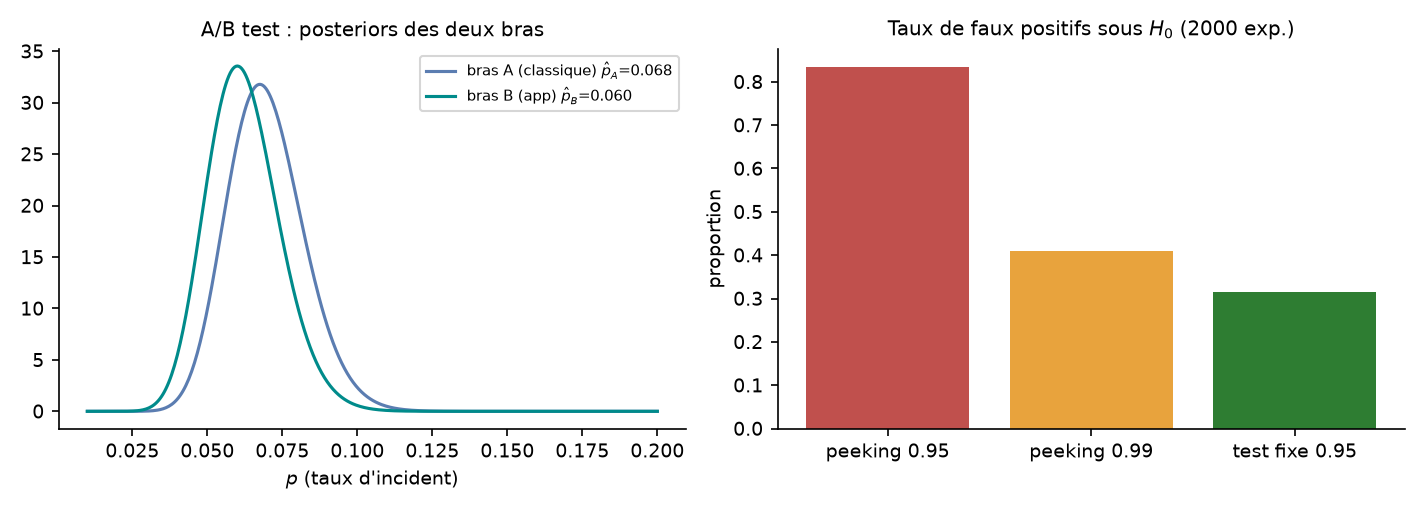
\includegraphics[width=0.72\textwidth]{fiche_ch4_abtest.png}
\end{center}

\textbf{Étape 3 --- la décision avec les coûts.} La direction chiffre :
appliquer l'appli coûte 1,5 MFCFA/an ; il reste 20~000 livraisons dans
l'année ; chaque point de réduction du taux vaut
$20\,000 \times 0{,}0421 = 842$ kFCFA par point. Le seuil de bascule
$\delta^{\star}$ (le gain moyen nécessaire pour rentabiliser l'appli) vaut
\[
\delta^{\star} = \frac{C_{\text{appli}}}{N_{\text{rest}} \times c_{\text{inc}}}
= \frac{1{,}5}{20\,000 \times 0{,}0421} \approx \textbf{0{,}18 point}
\]
soit $P(\Delta > \delta^{\star}) = \textbf{62{,}9~\%}$. L'espérance de gain
net de déployer l'appli vaut
\[
\mathbb{E}[\text{bénéfice net}] = P(\Delta > \delta^\star) \times
\mathbb{E}[\Delta \given \Delta > \delta^\star] \times N_{\text{rest}} \times c_{\text{inc}}
- C_{\text{appli}} \approx \textbf{+9{,}4 MFCFA} > 0.
\]
\textbf{Décision : déployer l'appli} --- même avec une certitude de seulement
63~\%, l'asymétrie des coûts (un faux pas coûte 1,5 MFCFA, rater un gain
réel coûte 3 à 4 fois plus) rend le déploiement rationnel. C'est l'exact
converse de la fiche 3 : là, la certitude était écrasante (99,4~\%) ; ici
elle est moyenne (63~\%), mais la \emph{structure des coûts} tranche.

\textbf{Étape 4 --- et l'espionnage ?} Si TransLog avait testé en fréquentiste
avec espionnage à chaque lot, environ 83~\% de ses « découvertes » seraient
des illusions. En bayésien, on ne promet pas de couverture long terme ; on
rapporte à chaque instant la probabilité que B batte A \emph{sur les
données réellement collectées} --- et on peut s'arrêter dès que le calcul de
coût le justifie, sans Gonfler le taux d'erreur.
\end{application}

\begin{qcmbox}[Questions 10 à 13]
\textbf{Q10.} $P(p_B > p_A) = 66{,}6~\%$ avec 400 livraisons par bras. Que
faut-il en conclure ?
\begin{enumerate}[label=\Alph*.), leftmargin=8mm, itemsep=0.3mm]
  \item l'appli est meilleure, c'est prouvé
  \item l'appli est plutôt meilleure, mais l'incertitude résiduelle est
        réelle (33~\% de masse contre) : la décision doit intégrer les coûts
        et éventuellement poursuivre la collecte
  \item le test a échoué, il faut recommencer
  \item la différence n'est pas « significative à 5~\% », donc il faut arrêter
\end{enumerate}

\vspace{2mm}
\textbf{Q11.} Le seuil de bascule $\delta^{\star} = 0{,}0018$ (0,18 point)
exprime :
\begin{enumerate}[label=\Alph*.), leftmargin=8mm, itemsep=0.3mm]
  \item le risque de première espèce maximal
  \item le gain moyen de taux au-delà duquel l'appli devient rentable, vu
        les coûts et le volume restant
  \item la ROPE du test A/B
  \item la moitié de l'écart-type de $\Delta$
\end{enumerate}

\vspace{2mm}
\textbf{Q12.} L'espérance de bénéfice net de déployer l'appli vaut +9,4 MFCFA
alors que $P(p_B > p_A)$ n'est que de 66,6~\%. L'explication est :
\begin{enumerate}[label=\Alph*.), leftmargin=8mm, itemsep=0.3mm]
  \item une erreur de calcul : on ne déploie jamais en dessous de 95~\%
  \item l'asymétrie des coûts : déployer à tort coûte 1,5 MFCFA, ne pas
        déployer à tort renonce à un gain espéré bien plus grand ; la
        décision optimale minimise le risque, elle ne cherche pas la
        certitude
  \item le volume de 20~000 livraisons compense mécaniquement
  \item les priors uniformes favorisent le bras B
\end{enumerate}

\vspace{2mm}
\textbf{Q13.} En fréquentiste, espionner le test à chaque lot avec
$\alpha = 0{,}05$ fait passer le taux de faux positifs nominal de 5~\% à
83,5~\%. Le test bayésien :
\begin{enumerate}[label=\Alph*.), leftmargin=8mm, itemsep=0.3mm]
  \item corrige automatiquement ce problème
  \item ne promet aucune couverture en répétition, donc la notion de « faux
        positifs gonflés » ne s'applique pas de la même façon ; mais il
        exige une honnêteté différente : rapporter la probabilité courante
        et justifier l'arrêt par le calcul des coûts
  \item est interdit par les régulateurs statistiques
  \item résout le problème en fixant $n$ à l'avance
\end{enumerate}
\end{qcmbox}

\begin{piege}[Questions 10 à 13]
\begin{itemize}[leftmargin=4mm, itemsep=0.5mm]
  \item \textbf{Q10} : « $P = 66{,}6~\%$ » n'est ni un verdict ni un échec :
        c'est une \emph{matière première pour la décision}. Le réflexe
        fréquentiste (« pas significatif, on arrête ») jette l'information
        de coût à la poubelle.
  \item \textbf{Q11} : le seuil de bascule n'est pas un seuil statistique
        mais un seuil \emph{économique} : il dépend du volume restant, du
        coût de l'appli et du coût d'incident. Changer un seul de ces trois
        paramètres change $\delta^\star$ --- d'où l'intérêt de le recalculer
        en continu.
  \item \textbf{Q12} : c'est le cœur philosophique du chapitre : la décision
        optimale n'est pas celle qui minimise la probabilité de se tromper,
        mais celle qui minimise l'\emph{espérance de perte}. Chercher la
        certitude avant d'agir, c'est payer un coût d'opportunité masqué.
  \item \textbf{Q13} : l'espionnage en fréquentiste est un vrai problème
        (l'inflation de $\alpha$ est réelle et documentée) ; la réponse
        bayésienne n'est pas une « correction » mais un changement de
        contrat : on renonce aux garanties en répétition contre une
        information décisionnelle à chaque instant. Les deux approches
        peuvent coexister : signaler les deux, choisir en connaissance de
        cause.
\end{itemize}
\end{piege}

% =====================================================================
%  SECTION 5 -- SYNTHESE
% =====================================================================
\section{Synthèse : les 5 réflexes à emporter (10 min)}

\begin{contexte}[Récapitulatif du dossier TransLog]
\begin{center}
\small
\begin{tabular}{@{}p{3.9cm} p{4.1cm} p{5.4cm}@{}}
\toprule
\textbf{Question business} & \textbf{Outil du chapitre 4} & \textbf{Réponse chiffrée} \\
\midrule
« La formation n'a rien changé » ? & facteur de Bayes (Savage--Dickey) & $BF_{10} = 7\,348$ : decisive \\
La $p$-value suffit-elle ? & borne de Sellke--Bayarri--Berger & $P(H_0) \ge 0{,}11~\%$ au mieux : non \\
Un modèle ou trois ? & LOO/WAIC + poids pseudo-BMA & M2 gagne ($\Delta = +1{,}33$ nats), poids 0,73 \\
Généraliser la formation ? & ROPE + espérance de perte & risque 25 vs 62 kFCFA : déployer \\
Déployer l'appli mobile ? & $P(p_B > p_A)$ + seuil de bascule & 66,6~\% de certitude, +9,4 MFCFA espérés \\
Espionner le test ? & inflation du taux de faux positifs & 83,5~\% de faux positifs à $\alpha = 0{,}05$ \\
\bottomrule
\end{tabular}
\end{center}

\textbf{Les 5 réflexes} à ancrer avant le chapitre 5 :
\begin{enumerate}[leftmargin=5mm, itemsep=1mm]
  \item \textbf{Une hypothèse se juge à ses prédictions} : le facteur de
        Bayes compare ce que chaque hypothèse \emph{prévoyait}, pas ce qu'elle
        « explique » après coup (4.1).
  \item \textbf{Un modèle se juge sur des données futures} : LOO/WAIC
        estiment le pouvoir prédictif, jamais l'ajustement passé (4.2).
  \item \textbf{La décision chiffre les erreurs} : ROPE pour la question
        pratique, espérance de perte pour le choix final --- toujours en
        unités qui parlent au décideur (4.3).
  \item \textbf{63~\% de certitude suffit si les coûts sont asymétriques} :
        la décision optimale minimise le risque, elle n'attend pas la
        certitude (4.4).
  \item \textbf{L'espionnage n'est pas neutre} : en fréquentiste, il détruit
        les garanties ; en bayésien, il exige de l'honnêteté (4.4).
\end{enumerate}
\end{contexte}

% =====================================================================
%  SECTION 6 -- QCM DE SYNTHESE (25 min)
% =====================================================================
\section{QCM de synthèse --- les réflexes transversaux (15 min)}

\begin{qcmbox}[Questions 14 et 15]
\textbf{Q14.} Le facteur de Bayes et la $p$-value s'accordent ici
(l'effet est réel pour les deux). Dans quel cas divergent-ils, et lequel
faire confiance ?
\begin{enumerate}[label=\Alph*.), leftmargin=8mm, itemsep=0.3mm]
  \item ils ne peuvent jamais diverger
  \item ils divergent quand la $p$-value est petite mais le prior sous $H_1$
        prédit mal les données ; le facteur de Bayes fait alors confiance à
        l'hypothèse qui prédit le mieux --- la $p$-value, elle, ne voit que
        l'écart à $H_0$
  \item ils divergent seulement pour $n < 30$
  \item la $p$-value est toujours plus fiable car sans prior
\end{enumerate}

\vspace{2mm}
\textbf{Q15.} TransLog résume le chapitre en une phrase pour son comité de
direction. La plus fidèle est :
\begin{enumerate}[label=\Alph*.), leftmargin=8mm, itemsep=0.3mm]
  \item « nos tests sont tous significatifs, nous pouvons tout déployer »
  \item « nous quantifions l'incertitude sur chaque hypothèse et chaque
        modèle, nous chiffrons ce que coûte chaque erreur, et nous choisissons
        l'action qui minimise l'espérance de perte --- même à 63~\% de
        certitude si les coûts le justifient »
  \item « le bayésien remplace la décision de la direction par un calcul »
  \item « nous comparons des modèles jusqu'à trouver celui qui colle
        parfaitement aux données »
\end{enumerate}
\end{qcmbox}

\begin{piege}[Questions 14 et 15]
\begin{itemize}[leftmargin=4mm, itemsep=0.5mm]
  \item \textbf{Q14} : la divergence $p$-value / facteur de Bayes survient
        quand le prior sous $H_1$ est mal calibré (cf.\ Q3 du volet 1 : le
        prior Beta(10,10) retourne le verdict). La $p$-value, elle, ne sait
        pas qu'un prior existe --- d'où son silence sur ce mécanisme.
  \item \textbf{Q15} : la bonne réponse décrit les \emph{trois étages} du
        chapitre : quantifier (facteurs de Bayes, elpd), chiffrer les erreurs
        (ROPE, coûts), décider (minimisation du risque). La réponse C est le
        piège symétrique de « la statistique décide à notre place » : le
        calcul éclaire la décision, la direction reste responsable.
\end{itemize}
\end{piege}

% =====================================================================
%  SECTION 7 -- CORRIGE
% =====================================================================
\newpage
\section{Corrigé complet des 15 QCM}

\begin{corrigebox}[Volet 1 --- le facteur de Bayes]
\textbf{Q1 : A.} Le facteur de Bayes $BF_{10} = p(y \given H_1)/p(y \given H_0)
= 7\,348$ compare les \textbf{vraisemblances marginales} : les données
observées sont 7~348 fois plus plausibles sous « la formation a changé
quelque chose » que sous « rien n'a changé ». La réponse B confond
vraisemblance et probabilité a posteriori (la conversion exige les
probabilités a priori des deux hypothèses) ; C confond avec la $p$-value
(qui vaut $4{,}1 \times 10^{-5}$, un tout autre objet) ; D confond avec la
masse du posterior hors de $p_0$ (qui vaut 99{,}998~\% et n'est pas un
facteur de Bayes).

\textbf{Q2 : B.} La borne de Sellke--Bayarri--Berger donne le \emph{plafond}
d'évidence qu'une $p$-value peut fournir : $BF_{10}^{\max} =
1/(-e\,p\ln p) = 889$ ici, et avec un prior neutre $P(H_0 \given y) \ge
\textbf{0{,}11~\%}$. Autrement dit, même dans le meilleur des mondes
bayésiens, une $p$-value de $4 \times 10^{-5}$ ne peut pas prouver que
$H_0$ a moins de 0,11~\% de chances d'être vraie. La réponse D (71~\%)
rappelle le chiffre du cours : pour une \emph{simple} $p = 0{,}05$ avec un
prior neutre, $P(H_0 \given y)$ peut monter à 71~\% --- l'écart entre la
$p$-value et la probabilité a posteriori est le message central du chapitre.

\textbf{Q3 : B.} Le prior Beta(10,10) prédit un taux de 50~\% ; les données
montrent 4,5~\%. Sous ce prior, l'hypothèse du concurrent (14,8~\%) prédit
les données \emph{mieux} que l'hypothèse « la formation marche » (qui se
retrouve coincée entre les deux). Le facteur de Bayes se retourne : ce n'est
pas un bug, c'est la mécanique de la vraisemblance marginale. La leçon
pratique : \textbf{publier l'analyse de sensibilité} --- le verdict avec
Beta(1,1) (2~400 en faveur de l'effet) et avec Beta(50,50) ($7{,}5\times
10^{13}$ en faveur de $H_0$) doit figurer côte à côte, jamais le seul
chiffre favori. Le facteur de Bayes reste utilisable (A est trop sévère) ;
Savage--Dickey est valable pour tout prior continu sous $H_1$ (C est faux) ;
modifier les données pour les faire concorder serait de la fraude (D).
\end{corrigebox}

\begin{corrigebox}[Volet 2 --- comparaison de modèles]
\textbf{Q4 : B.} L'elpd est une somme de \emph{log}-densités prédictives.
Une différence $\Delta\text{elpd} = +1{,}33$ nats en faveur de M2 correspond
à une vraisemblance marginale prédictive multipliée par $e^{1{,}33} \approx
\textbf{3{,}8}$. C'est le même réflexe que pour le facteur de Bayes : sur
l'échelle log, les écarts se convertissent en facteurs via l'exponentielle.
La réponse A lit l'écart brut comme un ratio --- erreur classique ;
C et D utilisent des conversions arbitraires sans justification.

\textbf{Q5 : B.} Le $p_{\text{waic}}$ mesure la \textbf{complexité effective}
: de combien le modèle « s'étire » pour épouser les données. Un modèle
nominalement à 1 paramètre ($\lambda$) avec un prior assez diffus et
seulement 6 observations peut avoir un $p_{\text{waic}} = 2{,}11$ : chaque
observation $y_i$ a « poussé » $\lambda$ dans une direction légèrement
différente, et le modèle a absorbé plus de flexibilité que son compte
nominal ne le suggère. C'est un signal utile (le prior pourrait être
resserré), pas une erreur (A), et ce n'est ni un compte d'observations (C)
ni un ajout de paramètres par le prior (D).

\textbf{Q6 : B.} Les poids pseudo-BMA transforment les elpd en poids sommant
à 1 : ici 0,19 / 0,73 / 0,07. La sagesse pratique est \textbf{double} :
(i) les poids rendent la comparaison \emph{auditable} --- on peut montrer au
comité que M2 concentre 73~\% de la plausibilité prédictive plutôt que
d'affirmer « M2 est le vrai modèle » ; (ii) quand aucun poids ne domine
(nettement sous 1), on \emph{combine} les modèles dans ces proportions
(empilement prédictif) plutôt que d'en choisir un seul. Ici, 0,73 domine
assez pour trancher avec M2 seul --- mais les poids restent l'outil de
communication. Jeter les autres modèles (A) jette de l'information ;
réfuter les données (C) ou moyenner des elpd (D) n'a pas de sens.
\end{corrigebox}

\begin{corrigebox}[Volet 3 --- ROPE et espérance de perte]
\textbf{Q7 : B.} La ROPE est fixée \emph{avant} de regarder les données, à
partir de la question pratique : « quel gain minimal justifie 2 MFCFA/an ? »
Ici $\pm 1$ point. Comme $P(\Delta > 0{,}01) = 99{,}998~\%$ et
$P(\Delta \in \text{ROPE}) < 0{,}01~\%$, \textbf{toute la masse posterior est
hors de la ROPE, du côté de l'effet réel} : la conclusion est univoque. Ce
n'est pas un test de significativité (A --- le seuil de 5~\% ne joue aucun
rôle), pas besoin d'atteindre exactement 95~\% (C), et la ROPE ne remplace
pas l'analyse de décision, elle l'amorce (D --- le calcul du risque vient
ensuite).

\textbf{Q8 : B.} Le risque bayésien d'une action $=$ espérance de sa perte,
où chaque scénario d'erreur est pondéré par la probabilité \emph{posterior}
qu'il se produise. Le coût de déployer à tort (2 MFCFA si l'effet était nul)
n'est encouru que sur la portion de posterior près de l'effet nul --- d'où un
risque espéré de 25,0 kFCFA seulement, alors que le coût brut est de 2 MFCFA
(\emph{sic} : les unités diffèrent, le risque est une espérance
annuelle pondérée). Ne pas déployer renonce au gain net sur la portion où
l'effet est réel --- d'où 62,3 kFCFA. Les réponses A, C, D ignorent cette
pondération par le posterior : ce sont des réflexes fréquentistes ou des
intuitions non chiffrées.

\textbf{Q9 : B.} L'objection « et si votre posterior est optimiste ? » est
la bonne question, et la bonne réponse est l'\textbf{analyse de robustesse} :
refaire le calcul de risque en dégradant volontairement le posterior (par
exemple en doublant la moyenne post-formation, donc en divisant $\Delta_E$
par deux). Le verdict bascule-t-il ? Ici non : même pessimiste, ne pas
déployer coûte plus cher que déployer, car le gain espéré (39,4 MFCFA) est
loin devant le coût de l'action (2 MFCFA). Répondre « mon chiffre est
objectif » (A) est un leurre --- tout posterior dépend d'un prior ; changer
la ROPE pour sauver la conclusion (C) est de la manipulation de critère ;
abandonner le bayésien (D) jette l'outil le plus adapté à la question posée.
\end{corrigebox}

\begin{corrigebox}[Volet 4 --- l'A/B test de l'appli mobile]
\textbf{Q10 : B.} $P(p_B > p_A) = 66{,}6~\%$ n'est ni une preuve (A --- un
tiers de la masse dit le contraire), ni un échec (C), ni une invitation à
appliquer un seuil de significativité (D --- ce seuil n'existe pas en
bayésien pur). C'est une \textbf{matière première décisionnelle} : elle
s'alimente dans le calcul des coûts (Q11--Q12) et peut argumenter une
poursuite de collecte si le gain espéré de continuer dépasse le coût
d'opportunité. C'est le mode de raisonnement bayésien appliqué : chiffres
$\to$ coûts $\to$ décision, jamais chiffres $\to$ verdict magique.

\textbf{Q11 : B.} Le seuil de bascule $\delta^{\star} = C_{\text{appli}} /
(N_{\text{rest}} \times c_{\text{inc}}) = 1{,}5 / (20\,000 \times 0{,}0421)
\approx 0{,}0018$ est un seuil \textbf{économique} : c'est le gain moyen de
taux au-delà duquel l'appli rembourse son coût. Il ne mesure ni un risque de
première espèce (A), ni une ROPE (C), ni une dispersion (D). Remarque
précieuse : $\delta^{\star}$ \emph{bouge} pendant le test, car
$N_{\text{rest}}$ diminue à chaque lot --- le seuil de rentabilité devient
plus exigeant au fil du temps, ce qui pousse naturellement vers une décision
plus tôt plutôt que plus tard.

\textbf{Q12 : B.} C'est la question philosophique du chapitre. Déployer à
tort coûte 1,5 MFCFA ; \emph{ne pas} déployer alors que l'appli fonctionne
renonce à $\Delta \times 20\,000 \times 0{,}0421$ --- plusieurs MFCFA pour
chaque point de réduction raté. Avec 66,6~\% de probabilité que B batte A,
l'espérance de gain net de déployer est positive (+9,4 MFCFA) : la
\textbf{structure des coûts} tranche là où la certitude ne suffit pas. La
réponse A (ne jamais déployer sous 95~\%) est le réflexe fréquentiste appliqué
hors de son domaine --- et ici, il coûterait de l'argent réel. C est
incomplet (le volume entre dans $\delta^\star$, mais l'explication complète
est l'asymétrie des coûts) ; D est faux (des priors uniformes ne favorisent
personne).

\textbf{Q13 : B.} L'espionnage fréquentiste (regarder à chaque lot, s'arrêter
dès que $p < \alpha$) gonfle massivement le taux de faux positifs : 83,5~\%
de « découvertes » fausses à $\alpha = 0{,}05$ sur A $=$ B. Le test bayésien
\emph{n'offre pas} de couverture en répétition (il ne promet rien sur le
long terme), donc la notion de « faux positifs gonflés » ne s'y applique pas
de la même façon --- mais il impose une \textbf{honnêteté différente} :
rapporter à chaque instant la probabilité courante que B batte A, et
justifier tout arrêt anticipé par le calcul des coûts, pas par « on a enfin
franchi le seuil ». Les réponses A et C sont des fausses sécurité ; D est
l'approche fréquentiste correcte (taille fixée à l'avance), mais elle renonce
à la flexibilité séquentielle que TransLog recherche.
\end{corrigebox}

\begin{corrigebox}[Volets 5 et synthèse --- réflexes transversaux]
\textbf{Q14 : B.} Facteur de Bayes et $p$-value s'accordent ici (les deux
disent « effet réel »), mais ils peuvent diverger : quand la $p$-value est
petite et que le prior sous $H_1$ prédit mal les données (ex.\ Q3 :
Beta(10,10) prédit 50~\%, les données montrent 4,5~\%), le facteur de Bayes
récompense l'hypothèse qui \emph{prédit} le mieux --- la $p$-value, elle, ne
sait mesurer que l'écart à $H_0$ et ignore complètement ce que $H_1$
prévoyait. La réponse D (« sans prior, donc plus fiable ») est exactement le
piège que le chapitre démonte : la $p$-value n'est pas « sans hypothèse »,
elle suppose implicitement que tout effet possible est aussi plausible ---
ce qui est déjà un choix de prior.

\textbf{Q15 : B.} La bonne réponse décrit les trois étages du chapitre :
\textbf{quantifier} (facteurs de Bayes, elpd, probabilités a posteriori),
\textbf{chiffrer les erreurs} (ROPE, coûts en FCFA), \textbf{décider}
(minimisation de l'espérance de perte). La réponse A est le résumé
fréquentiste parodié --- « tout est significatif » ignore précisément tout ce
que le chapitre a enseigné. C est le piège symétrique : le calcul éclaire,
la direction reste responsable. D est le piège du sur-ajustement : coller
aux données passées n'est jamais un critère de qualité d'un modèle --- le
pouvoir prédictif sur données futures l'est.
\end{corrigebox}

% =====================================================================
%  SECTION 8 -- POUR ALLER PLUS LOIN
% =====================================================================
\section{Pour aller plus loin}

\begin{contexte}[Après la fiche --- avant le chapitre 5]
\begin{itemize}[leftmargin=4mm, itemsep=1mm]
  \item \textbf{Relis les slides} : chapitre 4, sections 4.1 (facteur de
        Bayes et échelle de Jeffreys), 4.2 (comparaison LOO/WAIC),
        4.3 (ROPE et théorie de la décision), 4.4 (A/B testing et arrêt
        séquentiel). Chaque section correspond à un volet de cette fiche.
  \item \textbf{Rejoue les calculs} : le script \texttt{src/fiche\_ch4\_cameroun.py}
        régénère toutes les données du dossier (graine 4112) et les figures.
        Modifie le prior sous $H_1$ (par exemple $\text{Beta}(10, 10)$) et
        observe le retournement du facteur de Bayes --- c'est le meilleur
        entraînement possible sur la sensibilité au prior.
  \item \textbf{Prépare le chapitre 5} : le modèle par dépôt (M2) de cette
        fiche est un modèle \emph{indépendant} par groupe. Le chapitre 5
        introduit le modèle \textbf{hiérarchique} (M3 ici perdant, mais
        gagnant avec plus de dépôts) : lis la section 5.1 avant le prochain
        cours pour voir comment le partage partiel d'information entre
        groupes change la donne.
  \item \textbf{TP de rattrapage} : le notebook \texttt{TP4\_comparaison\_decision.ipynb}
        (répertoire \texttt{notebooks/}) te fait refaire toutes ces étapes en
        code, avec les mêmes données.
\end{itemize}
\end{contexte}

\end{document}
